The Rectified Linear Unit (RelU) is a very simple activation function, none the less, still a very useful function. When ReLU is called with some input, it will go through all values of the input, turning all negative values to 0, and all positive numbers simply keep their value.

$$
ReLU(input) = max(0,input)
$$
or
$$
ReLU(input) =
\left\{ \begin{matrix}
        input& \geq& 0& =& input& \\
        \\
        input& <& 0& =& 0&
\end{matrix}
\right.
$$


\begin{figure}[!ht]
  \centering
  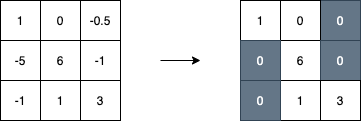
\includegraphics[scale=0.4]{latex/imgs/relu.png}
  \caption{Example of how ReLU() works}\label{Baseline:before}
\end{figure}
